\section{\trAnodyneMap{}与纤维化}
\label{sec:anodyne-maps-and-fibrations}

本节的目标是建立一些组合性的概念，使我们能够证明∞-\trGroupoid{}——即每个%
\trMorphism{}都可逆的\trInfinityCategories{}——事实上是\trKanComplex{}。对于%
空间∞-范畴与∞-\trCategories{}的\trInfinityCategory{}之定义而言，这些方法是核心所在。本节可视为该理论的
技术核心之一，我们将尽力给出一个简明的处理。我们从\trSaturatedSet{}（saturated set）的概念
出发，并讨论所谓\trQuillen{}\trSmallObjectArgument{}（small object argument）的一个特殊情形。
然后我们将利用这些结果证明：在\trSimplicialSets{}中可以施行的某些自然运算保持%
\trInfinityCategories{}与∞-\trGroupoid{}，其中最著名的是定理 1.3.37 及其推论。
由此，我们将对任意\trInfinityCategory{}中的任意两个\trObject{}，以典范的方式得到
二者之间的一个由\trMorphism{}构成的\trInfinityCategory{}。而证明这些由\trMorphism{}构成的%
∞-\trCategories{}事实上是∞-\trGroupoid{}，将是随后几节的内容。

\begin{definition}\label{def:fibration}
\trSimplicialSet{}之间的映射 $X \to Y$ 称为（内、左、右）\emph{纤维化}（fibration），若它对%
（内、左、右）\trHornInclusion{}满足\trRightLiftingProperty{}（right lifting property，RLP），如下图
所示
\begin{center}
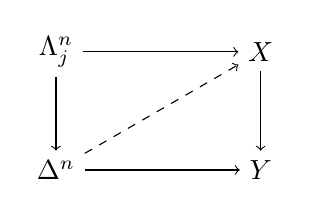
\begin{tikzpicture}
  \node (a) at (0,0) {$\Lambda^n_j$};
  \node (b) at (2.6,0) {$X$};
  \node (c) at (0,-1.5) {$\Delta^n$};
  \node (d) at (2.6,-1.5) {$Y$};
  \draw[->] (a) -- (b);
  \draw[->] (a) -- (c);
  \draw[->] (c) -- (d);
  \draw[->] (b) -- (d);
  \draw[->, dashed] (c) -- (b);
\end{tikzpicture}
\end{center}
\end{definition}

\begin{definition}\label{def:anodyne-map}
\trSimplicialSet{}之间的映射 $A \to B$ 称为（内、左、右）\emph{\trAnodyneMap{}}%
（anodyne map），若它对（内、左、右）纤维化满足\trLeftLiftingProperty{}（left lifting
property，LLP），如下图所示
\begin{center}
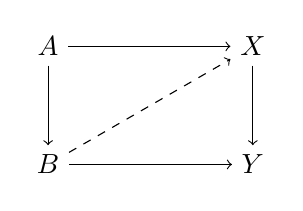
\begin{tikzpicture}
  \node (a) at (0,0) {$A$};
  \node (b) at (2.6,0) {$X$};
  \node (c) at (0,-1.5) {$B$};
  \node (d) at (2.6,-1.5) {$Y$};
  \draw[->] (a) -- (b);
  \draw[->] (a) -- (c);
  \draw[->] (c) -- (d);
  \draw[->] (b) -- (d);
  \draw[->, dashed] (c) -- (b);
\end{tikzpicture}
\end{center}
\end{definition}

\begin{definition}\label{def:chi}
设 $S$ 是\trCategory{} $\C$ 中的一集\trMorphism{}。我们令 $\chi_R(S)$ 为对 $S$ 满足
RLP 的那些\trMorphism{}所成之集，并令 $\chi_L(S)$ 为对 $S$ 满足 LLP 的那些%
\trMorphism{}所成之集。此外，我们令 $\chi(S) = \chi_L(\chi_R(S))$，也就是说，%
$\chi(S)$ 是由那些对「对 $S$ 满足 RLP 的\trMorphism{}」满足 LLP 的\trMorphism{}%
所成之集。
\end{definition}

\begin{example*}
设 $S$ 为（内、左、右）\trHornInclusion{}之集。则（内、左、右）纤维化由 $\chi_R(S)$
给出，而（内、左、右）\trAnodyneMap{}由 $\chi(S)$ 给出。
\end{example*}

接下来，我们想引入\trSimplicialSet{}的映射的\trSaturatedSet{}这一概念。为此，我们需要
下述定义。

\begin{definition}\label{def:retract}
设 $\C$ 是一个\trCategory{}。\trMorphism{} $f\colon A \to B$ 称为\trMorphism{}%
$f'\colon A' \to B'$ 的一个\emph{收缩}（retract），若存在交换图表
\begin{center}
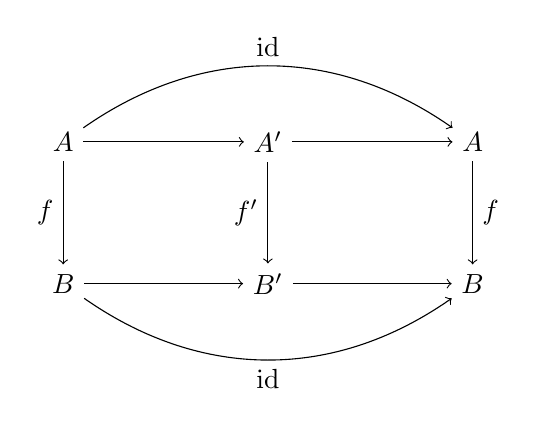
\begin{tikzpicture}
  \node (a1) at (0,0) {$A$};
  \node (a2) at (2.6,0) {$A'$};
  \node (a3) at (5.2,0) {$A$};
  \node (b1) at (0,-1.8) {$B$};
  \node (b2) at (2.6,-1.8) {$B'$};
  \node (b3) at (5.2,-1.8) {$B$};
  \draw[->] (a1) -- (a2);
  \draw[->] (a2) -- (a3);
  \draw[->] (b1) -- (b2);
  \draw[->] (b2) -- (b3);
  \draw[->] (a1) -- node[left] {$f$} (b1);
  \draw[->] (a2) -- node[left] {$f'$} (b2);
  \draw[->] (a3) -- node[right] {$f$} (b3);
  \draw[->, bend left=35] (a1) to node[above] {$\mathrm{id}$} (a3);
  \draw[->, bend right=35] (b1) to node[below] {$\mathrm{id}$} (b3);
\end{tikzpicture}
\end{center}
\end{definition}

\begin{definition}\label{def:saturated-set}
\trSimplicialSet{}的\trMorphism{}的一个\emph{\trSaturatedSet{}}（saturated set）是指一个对如下运算封闭的%
\trMorphism{}之集 $T$：取\trPushout{}（沿任意映射）、任意余积、可数合成（即沿
$\N$ 取\trColimit{}）以及收缩。给定任意一集\trMorphism{} $S$，我们把包含 $S$ 的
最小\trSaturatedSet{}称为 $S$ 的\emph{\trSaturation{}}（saturated closure），并记作
$\overline{S}$。
\end{definition}

\begin{remark}\label{rem:saturated-conditions}
让我们更精确地陈述\cref{def:saturated-set} 中诸条件之意：对任意余积封闭，是指给定
一族 $\{f_i\}_{i \in I}$，若每个 $f_i$ 都是 $T$ 的元素，则
$\amalg_{i \in I} f_i$ 也是 $T$ 的元素；对\trPushout{}封闭，是指给定属于 $T$ 的
映射 $f\colon A \to B$ 与任意其他映射 $\varphi\colon A \to A'$，则下面这个%
\trPushout{}图表中的映射 $f'$ 也属于 $T$：
\begin{center}
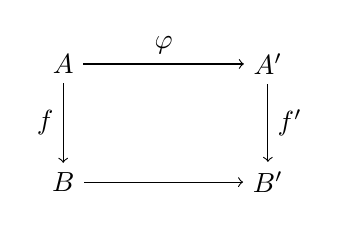
\begin{tikzpicture}
  \node (a) at (0,0) {$A$};
  \node (b) at (2.6,0) {$A'$};
  \node (c) at (0,-1.5) {$B$};
  \node (d) at (2.6,-1.5) {$B'$};
  \draw[->] (a) -- node[above] {$\varphi$} (b);
  \draw[->] (a) -- node[left] {$f$} (c);
  \draw[->] (b) -- node[right] {$f'$} (d);
  \draw[->] (c) -- (d);
\end{tikzpicture}
\end{center}
称 $T$ 对可数合成封闭，若对所有图表 $X\colon \N \to \mathrm{sSet}$，下述条件成立：
若对每个 $i \in \N$，映射
\[
X(i) \to X(i + 1)
\]
都含于 $T$，\footnote{译注：原书此处的「含于 $S$」与下文的「也含于 $S$」均按上下文
应为 $T$（该\trSaturatedSet{}）；「is contained is $S$」则为「is contained in $S$」之笔误。}
则映射 $X(0) \to \operatorname{colim}_{\N} X$ 也含于 $T$。最后，称 $T$ 对收缩封闭，
若对\cref{def:retract} 中的 $f$ 与 $f'$，当 $f'$ 是 $T$ 的元素时，$f$ 亦然。
\end{remark}

\begin{remark}\label{rem:saturated-closure-exists}
注意，\trSaturatedSet{}的交仍是\trSaturatedSet{}。因此，为看出\trSaturation{}存在，只需证明存在一个包含 $S$ 的%
\trSaturatedSet{}。例如，人们可以干脆取全体\trMorphism{}之集，它显然是\trSaturated{}且包含 $S$。
\end{remark}

\begin{example*}
$\mathrm{sSet}$ 中\trMonomorphism{}之集是一个\trSaturatedSet{}。
\end{example*}

\begin{lemma}\label{lem:chi-l-saturated}
给定一集\trMorphism{} $S$，我们有：$\chi_L(S)$ 是一个\trSaturatedSet{}。特别地，$\chi(S)$
是一个\trSaturatedSet{}。
\end{lemma}

\begin{proof}
设 $\alpha\colon A \to B$ 是 $\chi_L(S)$ 中的一个\trMorphism{}，并设
$\varphi\colon A \to A'$ 是任意一个\trMorphism{}。考虑\trPushout{}%
$B' = A' \amalg_A B$。我们希望证明典范映射 $A' \to B'$ 含于 $\chi_L(S)$。于是设
$f\colon X \to Y$ 是 $S$ 中的一个映射，并考虑图表
\begin{center}
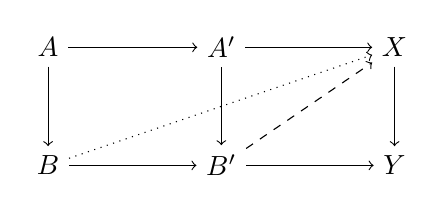
\begin{tikzpicture}
  \node (a1) at (0,0) {$A$};
  \node (a2) at (2.2,0) {$A'$};
  \node (a3) at (4.4,0) {$X$};
  \node (b1) at (0,-1.5) {$B$};
  \node (b2) at (2.2,-1.5) {$B'$};
  \node (b3) at (4.4,-1.5) {$Y$};
  \draw[->] (a1) -- (a2);
  \draw[->] (a2) -- (a3);
  \draw[->] (b1) -- (b2);
  \draw[->] (b2) -- (b3);
  \draw[->] (a1) -- (b1);
  \draw[->] (a2) -- (b2);
  \draw[->] (a3) -- (b3);
  \draw[->, dotted] (b1) -- (a3);
  \draw[->, dashed] (b2) -- (a3);
\end{tikzpicture}
\end{center}
其中我们希望构造出虚线映射。由假设，我们有点线映射，于是由\trPushout{}的泛性质
便得到虚线映射。同样地，设 $A \to B$ 是 $A' \to B'$ 的一个收缩，且 $A' \to B'$
含于 $\chi_L(S)$。为了证明此时 $A \to B$ 也含于 $\chi_L(S)$，我们取 $S$ 中的一个
映射 $f\colon X \to Y$ 与图表
\begin{center}
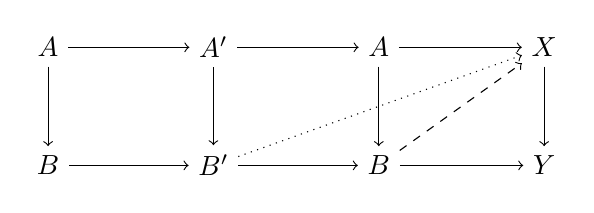
\begin{tikzpicture}
  \node (a1) at (0,0) {$A$};
  \node (a2) at (2.1,0) {$A'$};
  \node (a3) at (4.2,0) {$A$};
  \node (a4) at (6.3,0) {$X$};
  \node (b1) at (0,-1.5) {$B$};
  \node (b2) at (2.1,-1.5) {$B'$};
  \node (b3) at (4.2,-1.5) {$B$};
  \node (b4) at (6.3,-1.5) {$Y$};
  \draw[->] (a1) -- (a2);
  \draw[->] (a2) -- (a3);
  \draw[->] (a3) -- (a4);
  \draw[->] (b1) -- (b2);
  \draw[->] (b2) -- (b3);
  \draw[->] (b3) -- (b4);
  \draw[->] (a1) -- (b1);
  \draw[->] (a2) -- (b2);
  \draw[->] (a3) -- (b3);
  \draw[->] (a4) -- (b4);
  \draw[->, dotted] (b2) -- (a4);
  \draw[->, dashed] (b3) -- (a4);
\end{tikzpicture}
\end{center}
其中我们希望证明虚线箭头存在。同样，点线箭头存在，而且我们可沿映射 $B \to B'$
将其拉回到 $B$ 上。

现在设给定了一族 $\{f_i\colon A_i \to B_i\}_{i \in I}$，其元素都属于
$\chi_L(S)$。我们于是要证 $\amalg_{i \in I} f_i \in \chi_L(S)$ 也成立。为此，
考虑\trLiftingProblem{}%
\begin{center}
\begin{tikzpicture}
  \node (t) at (0,0) {$\amalg_{i \in I} A_i$};
  \node (r) at (3.2,0) {$X$};
  \node (l) at (0,-2.2) {$\amalg_{i \in I} B_i$};
  \node (b) at (3.2,-2.2) {$Y$};
  \draw[->] (t) -- (r);
  \draw[->] (t) -- node[left] {$\underset{i \in I}{\amalg} f_i$} (l);
  \draw[->] (l) -- (b);
  \draw[->] (r) -- node[right] {$\varphi$} (b);
  \draw[->, dashed] (l) -- (r);
\end{tikzpicture}
\end{center}
其中 $\varphi\colon X \to Y$ 是 $S$ 的一个元素。那么虚线箭头的存在由余积的泛性质
以及「每个 $f_i$ 都是 $\chi_L(S)$ 的元素」这一假设立得。

剩下要证明：对任何图表 $A\colon \N \to \C$，若每个映射 $A_i \to A_{i+1}$ 都含于
$\chi_L(S)$，则映射 $A_0 \to A = \operatorname{colim}_i A_i$ 也含于
$\chi_L(S)$。\footnote{译注：原书印作「$\operatorname{colim}_i X_i$」，但此处
图表名为 $A$，按上下文应为 $A_i$。}这由\trColimit{}的泛性质简单得出：我们再取
$S$ 中的 $f\colon X \to Y$ 与图表
\begin{center}
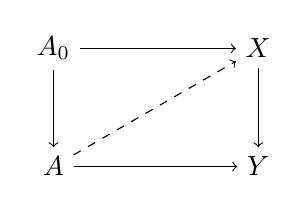
\begin{tikzpicture}
  \node (t) at (0,0) {$A_0$};
  \node (r) at (2.6,0) {$X$};
  \node (l) at (0,-1.5) {$A$};
  \node (b) at (2.6,-1.5) {$Y$};
  \draw[->] (t) -- (r);
  \draw[->] (t) -- (l);
  \draw[->] (l) -- (b);
  \draw[->] (r) -- (b);
  \draw[->, dashed] (l) -- (r);
\end{tikzpicture}
\end{center}
其中我们需要证明虚线箭头存在。由于这是一个从\trColimit{}出发的映射，只需证明存在
彼此相容的映射 $A_i \to X$ 使得一切交换。而这可以归纳地完成，所利用的事实是每个
映射 $A_i \to A_{i+1}$ 都含于 $\chi_L(S)$。
\end{proof}

下述结果被称为\emph{\trSmallObjectArgument{}}（small object argument）。它是构造映射的非平凡
分解的一个非常有用的工具。

\begin{proposition}\label{prop:small-object-argument}
设 $S$ 是\trSimplicialSet{}的\trMorphism{}之集 $\{A_i \to B_i\}_{i \in I}$，使得对每个
$i \in I$，\trSimplicialSet{} $A_i$ 只有有限多个非退化\trSimplex{}。若 $f$ 是任意一个\trMorphism{}，
则 $f$ 可以分解成一个含于 $\overline{S}$ 的映射与一个对 $S$ 具有 RLP 的映射的
复合。
\end{proposition}

\begin{proof}
首先，考虑由三元组 $(\alpha_i, u_i, v_i)$ 构成的集合 $\Theta_S$，其中
$\alpha_i\colon A_i \to B_i$ 是 $S$ 的一个元素，而 $u_i\colon A_i \to X$ 与
$v_i\colon B_i \to Y$ 是使图表
\begin{center}
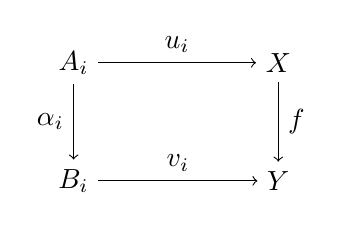
\begin{tikzpicture}
  \node (t) at (0,0) {$A_i$};
  \node (r) at (2.6,0) {$X$};
  \node (l) at (0,-1.5) {$B_i$};
  \node (b) at (2.6,-1.5) {$Y$};
  \draw[->] (t) -- node[above] {$u_i$} (r);
  \draw[->] (t) -- node[left] {$\alpha_i$} (l);
  \draw[->] (l) -- node[above] {$v_i$} (b);
  \draw[->] (r) -- node[right] {$f$} (b);
\end{tikzpicture}
\end{center}
交换的映射。我们得到一个交换图表
\begin{center}
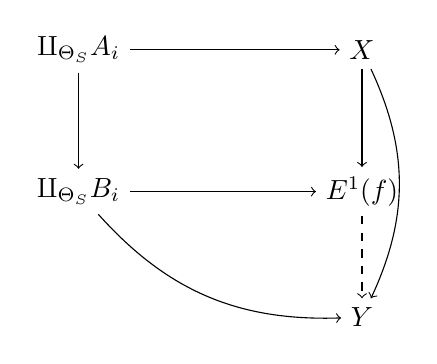
\begin{tikzpicture}
  \node (al) at (0,0) {$\amalg_{\Theta_S} A_i$};
  \node (x) at (3.6,0) {$X$};
  \node (bl) at (0,-1.8) {$\amalg_{\Theta_S} B_i$};
  \node (e) at (3.6,-1.8) {$E^1(f)$};
  \node (y) at (3.6,-3.4) {$Y$};
  \draw[->] (al) -- (x);
  \draw[->] (bl) -- (e);
  \draw[->] (al) -- (bl);
  \draw[->] (x) -- (e);
  \draw[->] (x) to[bend left=25] (y);
  \draw[->] (bl) to[bend right=25] (y);
  \draw[->, dashed] (e) -- (y);
\end{tikzpicture}
\end{center}
其中 $E^1(f)$ 定义为该\trPushout{}。由于 $\overline{S}$ 对小余积与\trPushout{}%
封闭，我们可以推出映射 $X \to E^1(f)$ 含于 $\overline{S}$。

对映射 $E^1(f) \to Y$ 施行与刚才对映射 $f\colon X \to Y$ 所做的同样的操作，我们便
得到一个序列
\[
X \to E^1(f) \to E^2(f) \to \dotsb \to Y.
\]
令 $E^{\omega}(f) = \operatorname{colim}_k E^k(f)$，其中 $\omega$ 用作第一个极限
序数的记号，于是我们得到一个分解
\[
X \to E^{\omega}(f) \to Y.
\]
由构造，每个映射 $E^k(f) \to E^{k+1}(f)$ 都含于 $\overline{S}$，因为
$\overline{S}$ 对\trPushout{}与余积封闭。因此，由于 $\overline{S}$ 是\trSaturated{}，
映射 $X \to E^{\omega}(f)$ 也含于 $\overline{S}$。剩下要证映射
$E^{\omega}(f) \to Y$ 含于 $\chi_R(S)$。为此，让我们考虑 $S$ 中的一个映射
$A_i \to B_i$ 与图表
\begin{center}
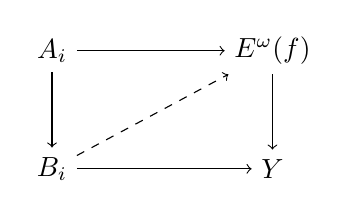
\begin{tikzpicture}
  \node (t) at (0,0) {$A_i$};
  \node (r) at (2.8,0) {$E^{\omega}(f)$};
  \node (l) at (0,-1.5) {$B_i$};
  \node (b) at (2.8,-1.5) {$Y$};
  \draw[->] (t) -- (r);
  \draw[->] (t) -- (l);
  \draw[->] (l) -- (b);
  \draw[->] (r) -- (b);
  \draw[->, dashed] (l) -- (r);
\end{tikzpicture}
\end{center}
其中我们希望证明虚线箭头存在，它将使两个三角形都交换。现在我们断言：典范映射
\[
\operatorname{colim}_{k \in \N}
\mathrm{Hom}_{\mathrm{sSet}}(A_i, E^k(f)) \to
\mathrm{Hom}_{\mathrm{sSet}}(A_i, E^{\omega}(f))
\]
是双射。（事实上，这样的 $A_i$ 是\emph{\trCompact{}}（compact），也就是说，
$\mathrm{Hom}_{\mathrm{sSet}}(A_i, -)$ 与一般的\trFiltered{}%
\trColimit{}交换。）这由「$A_i$ 中只有有限多个非退化\trSimplex{}」以及「任何单纯映射被它
在非退化\trSimplex{}上的取值所确定」这两个事实得出。因此，我们找到 $k \in \N$ 使得给定的
映射 $A_i \to E^{\omega}(f)$ 分解为复合
\[
A_i \to E^k(f) \to E^{\omega}(f).
\]
现在图表
\begin{center}
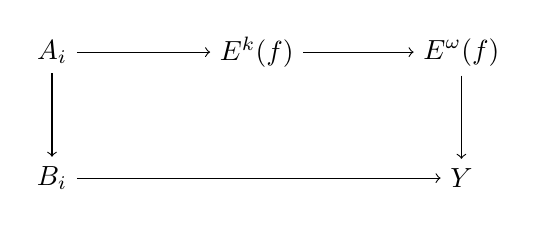
\begin{tikzpicture}
  \node (a) at (0,0) {$A_i$};
  \node (m) at (2.6,0) {$E^k(f)$};
  \node (r) at (5.2,0) {$E^{\omega}(f)$};
  \node (b1) at (0,-1.6) {$B_i$};
  \node (b2) at (5.2,-1.6) {$Y$};
  \draw[->] (a) -- (m);
  \draw[->] (m) -- (r);
  \draw[->] (a) -- (b1);
  \draw[->] (r) -- (b2);
  \draw[->] (b1) -- (b2);
\end{tikzpicture}
\end{center}
交换，于是由 $E^{k+1}(f)$ 的定义本身，存在交换图表
\begin{center}
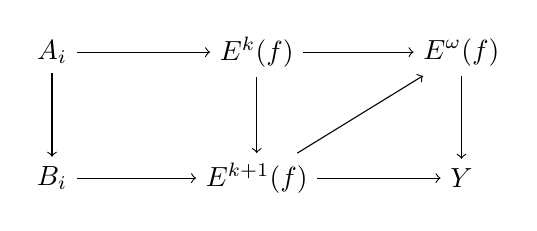
\begin{tikzpicture}
  \node (a) at (0,0) {$A_i$};
  \node (m) at (2.6,0) {$E^k(f)$};
  \node (r) at (5.2,0) {$E^{\omega}(f)$};
  \node (b1) at (0,-1.6) {$B_i$};
  \node (bm) at (2.6,-1.6) {$E^{k+1}(f)$};
  \node (b2) at (5.2,-1.6) {$Y$};
  \draw[->] (a) -- (m);
  \draw[->] (m) -- (r);
  \draw[->] (a) -- (b1);
  \draw[->] (m) -- (bm);
  \draw[->] (r) -- (b2);
  \draw[->] (b1) -- (bm);
  \draw[->] (bm) -- (b2);
  \draw[->] (bm) -- (r);
\end{tikzpicture}
\end{center}
它解决了我们的\trLiftingProblem{}。
\end{proof}

\begin{remark}\label{rem:small-object-size}
本书中用于\trSmallObjectArgument{}的那些\trSimplicialSet{} $A_i$ 将只有有限多个非退化\trSimplex{}。一般地，我们将
不得不寻找一个正则基数 $\kappa$，它大于 $S$ 中出现的任何一个 $A_i$ 的基数（这
保证所有 $A_i$ 确实是 $\kappa$-\trCompact{}）。此外，我们将不得不把\trSaturatedSet{}定义为对任意
序数上取指标的\trColimit{}封闭，而不只是对序数 $\omega$ 封闭。然后我们可以延续
上面的归纳过程，即在后继序数处像之前那样考虑\trPushout{}，而在极限序数处像之前
那样取\trColimit{}。进行到某一步，人们便定义了 $E^{\kappa}(f)$，它坐落于一个分解
$X \to E^{\kappa}(f) \to Y$ 之中，而一个与之前类似的论证将表明：第一个映射含于
$\overline{S}$（按\trSaturatedSet{}的新定义），且后一个映射含于 $\chi_R(S)$。本书选择不去
处理序数上的\trColimit{}，因为我们用不着它。但是，知道\trSmallObjectArgument{}并不依赖于这类
大小问题，当然是有益的。
\end{remark}

\begin{remark}\label{rem:small-object-functorial}
如上所述的分解是\trFunctor{}性的：每当给定一个交换图表
\begin{center}
\begin{tikzpicture}
  \node (t1) at (0,0) {$X$};
  \node (t2) at (2.4,0) {$Y$};
  \node (b1) at (0,-1.5) {$X'$};
  \node (b2) at (2.4,-1.5) {$Y'$};
  \draw[->] (t1) -- node[above] {$f$} (t2);
  \draw[->] (t1) -- (b1);
  \draw[->] (t2) -- (b2);
  \draw[->] (b1) -- node[above] {$f'$} (b2);
\end{tikzpicture}
\end{center}
\trSmallObjectArgument{}事实上就提供一个交换图表
\begin{center}
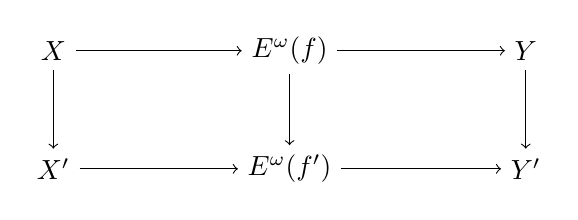
\begin{tikzpicture}
  \node (t1) at (0,0) {$X$};
  \node (t2) at (3,0) {$E^{\omega}(f)$};
  \node (t3) at (6,0) {$Y$};
  \node (b1) at (0,-1.5) {$X'$};
  \node (b2) at (3,-1.5) {$E^{\omega}(f')$};
  \node (b3) at (6,-1.5) {$Y'$};
  \draw[->] (t1) -- (t2);
  \draw[->] (t2) -- (t3);
  \draw[->] (t1) -- (b1);
  \draw[->] (t2) -- (b2);
  \draw[->] (t3) -- (b3);
  \draw[->] (b1) -- (b2);
  \draw[->] (b2) -- (b3);
\end{tikzpicture}
\end{center}
\end{remark}

借助\trSmallObjectArgument{}，我们现在可以给出\cref{prop:infinity-category-composer} 的一个证明。
（注意，也可以给出一个直接的证明。）

\begin{proposition}\label{prop:spine-closure-not-inner-anodyne}
由\trSpineInclusion{}生成的\trSaturatedSet{}不等于\trInnerAnodyne{}映射。此外，存在不是%
\trInfinityCategory{}的\trComposer{}。
\end{proposition}

\begin{proof}
考虑包含 $\Lambda^3_1 \to \Delta^3$。由\trSmallObjectArgument{}，我们可以把这个映射分解成复合
\[
\Lambda^3_1 \to X \to \Delta^3
\]
使得第一个映射位于由\trSpineInclusion{}生成的\trSaturatedClass{}之中，而最后一个映射对\trSpineInclusion{}%
满足 RLP，从而也对由\trSpineInclusion{}生成的\trSaturatedSet{}满足 RLP。由此得出 $X$ 是一个%
\trComposer{}，因为映射 $\Delta^3 \to \Delta^0$ 也对\trSpineInclusion{}满足 RLP。如果
由\trSpineInclusion{}生成的\trSaturatedSet{}等于\trInnerAnodyne{}映射，那么就会得出映射
$X \to \Delta^3$ 是一个\trInnerFibration{}（因为它对\trInnerAnodyne{}映射满足
RLP）。我们将证明情况并非如此。为此，我们断言：\trLiftingProblem{}%
\begin{center}
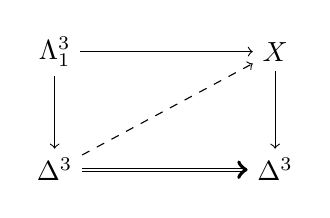
\begin{tikzpicture}
  \node (t) at (0,0) {$\Lambda^3_1$};
  \node (r) at (2.8,0) {$X$};
  \node (l) at (0,-1.5) {$\Delta^3$};
  \node (b) at (2.8,-1.5) {$\Delta^3$};
  \draw[->] (t) -- (r);
  \draw[->] (t) -- (l);
  \draw[double, ->] (l) -- (b);
  \draw[->] (r) -- (b);
  \draw[->, dashed] (l) -- (r);
\end{tikzpicture}
\end{center}
无解。这可以通过对 $X$ 上由\trSmallObjectArgument{}得到的滤过作归纳而轻易证明，所用的观察是：
给定\trSimplicialSet{}的一个\trPushout{}%
\begin{center}
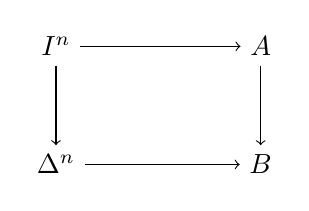
\begin{tikzpicture}
  \node (t) at (0,0) {$I^n$};
  \node (r) at (2.6,0) {$A$};
  \node (l) at (0,-1.5) {$\Delta^n$};
  \node (b) at (2.6,-1.5) {$B$};
  \draw[->] (t) -- (r);
  \draw[->] (t) -- (l);
  \draw[->] (l) -- (b);
  \draw[->] (r) -- (b);
\end{tikzpicture}
\end{center}
其中 $n \ge 3$，那么 $\Lambda^n_j \subseteq \Delta^n$ 在 $B$ 中的像不含于 $A$
之中。

若 $X$ 是一个\trInfinityCategory{}，则映射 $X \to \Delta^3$ 确实会是一个%
\trInnerFibration{}，见\cref{ex:inner-fibration-op}。但我们已经证明它不是。
\end{proof}

\begin{remark}\label{rem:alternative-composer-argument}
本命题也可以由另一个论证得出：结合\cref{ex:coherent-nerve-existence} 与\cref{lem:coherent-nerve-composer}，
我们看到存在不是\trInfinityCategory{}的\trComposer{} $X$。现在，映射
$X \to \Delta^0$ 含于 $\chi_R(\{I^n \to \Delta^n\}_{n \in \N})$，但它不是一个%
\trInnerFibration{}。这表明\trSpineInclusion{}的\trSaturation{}不可能由\trInnerAnodyne{}映射
给出，因为否则任何对\trSpineInclusion{}满足 RLP 的映射也将是一个\trInnerFibration{}。

注意，单凭「\trSpineInclusion{}的\trSaturation{}不等于\trInnerAnodyne{}映射」这一事实，并不
形式地蕴含「存在不是\trInfinityCategory{}的\trComposer{}」。然而，反过来的蕴含
成立：不是\trInfinityCategory{}的\trComposer{}的存在表明，由\trSpineInclusion{}生成的%
\trSaturatedSet{}不可能包含全部\trInnerAnodyne{}映射。
\end{remark}

\begin{remark}\label{rem:spine-inner-anodyne-restated}
我们将在\cref{prop:spine-inner-anodyne} 中证明\trSpineInclusion{}是\trInnerAnodyne{}的，
于是\cref{prop:spine-closure-not-inner-anodyne} 可以重新陈述为：由\trSpineInclusion{}%
生成的\trSaturatedSet{}真含于\trInnerAnodyne{}映射之中。
\end{remark}

\begin{lemma}\label{lem:saturated-closure-equals-chi}
考虑一集\trMorphism{} $S = \{A_i \to B_i\}_{i \in I}$，使得所有 $A_i$ 都只有
有限多个非退化\trSimplex{}。那么 $S$ 的\trSaturation{} $\overline{S}$ 由 $\chi(S)$ 给出。
\end{lemma}

\begin{proof}
显然，我们有 $S \subseteq \chi(S)$。在\cref{lem:chi-l-saturated} 中我们已经证明
$\chi(S)$ 自身是\trSaturated{}，因此 $\overline{S} \subseteq \chi(S)$。为了证明反包含，
考虑映射 $f\colon x \to y$，其中 $f \in \chi(S)$。由%
\cref{prop:small-object-argument} 的\trSmallObjectArgument{}，我们找到该映射的一个分解
\begin{center}
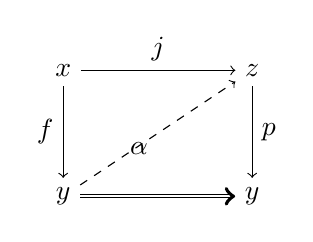
\begin{tikzpicture}
  \node (t) at (0,0) {$x$};
  \node (r) at (2.4,0) {$z$};
  \node (l) at (0,-1.6) {$y$};
  \node (b) at (2.4,-1.6) {$y$};
  \draw[->] (t) -- node[above] {$j$} (r);
  \draw[->] (t) -- node[left] {$f$} (l);
  \draw[double, ->] (l) -- (b);
  \draw[->] (r) -- node[right] {$p$} (b);
  \draw[->, dashed] (l) -- node[below left] {$\alpha$} (r);
\end{tikzpicture}
\end{center}
其中 $j \in \overline{S}$，而 $p$ 对 $S$ 满足 RLP。由于 $f \in \chi(S)$，由此
得出存在虚线箭头 $\alpha$，它使图表交换。于是，我们有交换图表
\begin{center}
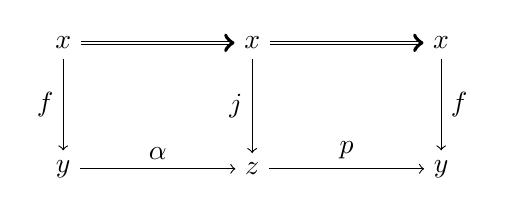
\begin{tikzpicture}
  \node (a1) at (0,0) {$x$};
  \node (a2) at (2.4,0) {$x$};
  \node (a3) at (4.8,0) {$x$};
  \node (b1) at (0,-1.6) {$y$};
  \node (b2) at (2.4,-1.6) {$z$};
  \node (b3) at (4.8,-1.6) {$y$};
  \draw[double, ->] (a1) -- (a2);
  \draw[double, ->] (a2) -- (a3);
  \draw[->] (a1) -- node[left] {$f$} (b1);
  \draw[->] (a2) -- node[left] {$j$} (b2);
  \draw[->] (a3) -- node[right] {$f$} (b3);
  \draw[->] (b1) -- node[above] {$\alpha$} (b2);
  \draw[->] (b2) -- node[above] {$p$} (b3);
\end{tikzpicture}
\end{center}
它表明 $f$ 是 $j$ 的一个收缩。由于 $j \in \overline{S}$，同样的结论也适用于
$f$。
\end{proof}

\begin{corollary}\label{cor:anodyne-saturated-closure}
（内、左、右）\trAnodyneMap{}恰好是（内、左、右）\trHornInclusion{}的\trSaturation{}。特别地，
它们全部都是\trMonomorphism{}。
\end{corollary}

作为\cref{fact:anodyne-extension} 的一个扩充，我们还记录下如下事实。

\begin{fact}\label{fact:anodyne-iff-realization-we}
一个\trMonomorphism{}是\trAnodyne{}的，当且仅当它的\trGeometricRealization{}是一个%
\trWeakEquivalence{}。这是\trSimplicialSet{}上 Kan--\trQuillen{}\trModelStructure{}之存在性的一部分
\cite[Theorem 11.3]{GJ09}，该\trModelStructure{}等价于拓扑空间上的\trQuillen{}\trModelStructure{}。
\end{fact}

下面的推论是\cref{lem:coherent-nerve-composer} 的相对版本。

\begin{corollary}\label{cor:relative-nerve-inner-fibration}
设 $F\colon \C \to \D$ 是单纯\trCategories{}之间的一个\trMorphism{}。假设
对所有\trObject{} $X, Y \in \C$，诱导映射
$\mathrm{Hom}_{\C}(X, Y) \to \mathrm{Hom}_{\D}(FX, FY)$ 是一个%
\trKanFibration{}。那么
$\mathrm{N}F\colon \mathrm{N}\C \to \mathrm{N}\D$ 是一个%
\trInnerFibration{}。
\end{corollary}

\begin{corollary}\label{cor:nerve-functor-inner-fibration}
设 $F\colon \C \to \D$ 是普通\trCategories{}之间的一个\trFunctor{}。那么
诱导\trFunctor{} $\mathrm{N}F\colon \mathrm{N}\C \to \mathrm{N}\D$ 是一个%
\trInnerFibration{}。
\end{corollary}

\begin{proof}
给定集合之间的任意映射 $A \to B$，常值\trSimplicialSet{}的诱导映射 $cA \to cB$ 是一个%
\trKanFibration{}。这由如下事实得出：对所有 $n \ge 1$ 与所有 $0 \le j \le n$，
映射 $\pi_0(\Lambda^n_j) \to \pi_0(\Delta^n)$ 是同构。然后用
$\mathrm{N}(\C) = \mathrm{N}(c\C)$ 这一事实与上一个推论即可完成证明。
\end{proof}

\begin{remark}\label{rem:inner-fibration-characterization}
事实上，更多的结论成立：\cref{ex:inner-fibration-op} 中证明了，\trSimplicialSet{}之间的映射
$X \to \mathrm{N}(\D)$（其中 $\D$ 是普通\trCategory{}）是一个%
\trInnerFibration{}，当且仅当 $X$ 是一个\trInfinityCategory{}。
\end{remark}

为了接下来的内容，我们必须回顾\cref{def:boundary-horn-spine} 中 $S$-\trHorn{}%
$\Lambda^n_S$ 的定义，即有
\[
\Lambda^n_S = \bigcup_{s \notin S} \Delta^{[n]\setminus\{s\}}.
\]

\begin{lemma}\label{lem:s-horn-anodyne}
设 $S \subseteq [n]$ 是一个非空子集。那么映射 $\Lambda^n_S \to \Delta^n$ 是
\begin{enumerate}[label=(\arabic*)]
  \item \trAnodyne{}的，只要 $S \ne [n]$；
  \item \trLeftAnodyne{}的，只要 $\{n\} \notin S$；
  \item \trRightAnodyne{}的，只要 $\{0\} \notin S$；
  \item \trInnerAnodyne{}的，只要 $S$ 不是某个区间的补集，也就是说，存在
  $a < b < c \in [n]$ 使 $a, c \notin S$ 但 $b \in S$。
\end{enumerate}
\end{lemma}

\begin{proof}
设 $S \subseteq [n]$ 是非空子集，设 $s \in S$ 并令 $S' = S \setminus \{s\}$。
考虑\trPushout{}图表
\begin{center}
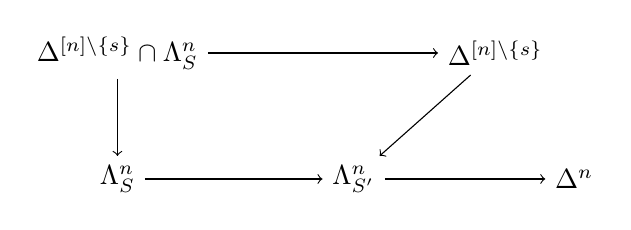
\begin{tikzpicture}
  \node (tl) at (0,0) {$\Delta^{[n]\setminus\{s\}} \cap \Lambda^n_S$};
  \node (tr) at (4.8,0) {$\Delta^{[n]\setminus\{s\}}$};
  \node (bl) at (0,-1.6) {$\Lambda^n_S$};
  \node (bm) at (3,-1.6) {$\Lambda^n_{S'}$};
  \node (br) at (5.8,-1.6) {$\Delta^n$};
  \draw[->] (tl) -- (tr);
  \draw[->] (tl) -- (bl);
  \draw[->] (tr) -- (bm);
  \draw[->] (bl) -- (bm);
  \draw[->] (bm) -- (br);
\end{tikzpicture}
\end{center}
注意，上面的水平箭头是一个广义\trHornInclusion{}%
$\Lambda^{[n]\setminus\{s\}}_{S'} \subseteq \Delta^{[n]\setminus\{s\}}$。由此
得出，包含 $\Lambda^n_S \to \Delta^n$ 含于由诸包含
$\Lambda^{[n]\setminus\{s\}}_{S'} \subseteq \Delta^{[n]\setminus\{s\}}$ 与
$\Lambda^n_{S'} \subseteq \Delta^n$ 生成的最小\trSaturatedSet{}之中。

我们将对 $S$ 的大小（对任意的 $[n]$）作归纳来证明本引理。让我们先考虑（1）。若
$S$ 只含一个元素，比如说 $S = \{i\}$，则 $\Lambda^n_S$ 是一个\trHornInclusion{}，从而
是\trAnodyne{}的。若 $S$ 含有多于一个元素，则 $S'$ 仍至少含一个元素且比 $S$ 小，于是
$\Lambda^n_{S'} \subseteq \Delta^n$ 与
$\Lambda^{[n]\setminus\{s\}}_{S'} \subseteq \Delta^n$ 由归纳
是\trAnodyne{}的。

对于（2），设 $S = \{i\}$。则该\trHornInclusion{}是\trLeftAnodyne{}的，因为 $i \ne n$。若 $S$
含有多于一个元素，则 $S'$ 更小且仍不含 $n$。（3）的陈述是类似的。

为了证明（4），我们首先注意：若 $S = \{i\}$，则必有 $0 < i < n$，否则其补集是
一个区间，于是包含 $\Lambda^n_S \to \Delta^n$ 是\trInnerAnodyne{}的。若 $S$ 含有多于一个
元素，则我们断言：存在 $S$ 中的元素 $s$ 使得 $S \setminus \{s\}$ 仍不是某个区间
的补集：由假设，存在 $a < b < c$ 使 $b \in S$ 且 $a, c \notin S$；而同样由
假设，$S \ne \{b\}$，故可以选取另一个元素 $s \in S \setminus \{b\}$。那么
$S' = S \setminus \{s\}$ 仍不是某个区间的补集（因为 $b \in S'$）。
\end{proof}

\begin{proposition}\label{prop:spine-inner-anodyne}
\trSpineInclusion{} $I^n \to \Delta^n$ 是\trInnerAnodyne{}的。
\end{proposition}

\begin{proof}
\trSpineInclusion{} $i_n\colon I^n \to \Delta^n$ 可以作如下分解：
\[
I^n \xrightarrow{\ f_n\ } \Delta^{[n]\setminus\{0\}} \cup I^n
\xrightarrow{\ g_n\ } \Delta^n
\]
我们将对 $n$ 作归纳证明 $f_n$ 与 $g_n$ 都是\trInnerAnodyne{}的。归纳起步 $n = 1$ 与 $n = 2$
是显然的。现在设 $n \ge 3$，考虑\trPushout{}图表
\begin{center}
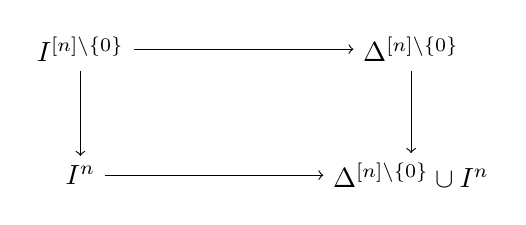
\begin{tikzpicture}
  \node (tl) at (0,0) {$I^{[n]\setminus\{0\}}$};
  \node (tr) at (4.2,0) {$\Delta^{[n]\setminus\{0\}}$};
  \node (bl) at (0,-1.6) {$I^n$};
  \node (br) at (4.2,-1.6) {$\Delta^{[n]\setminus\{0\}} \cup I^n$};
  \draw[->] (tl) -- (tr);
  \draw[->] (tl) -- (bl);
  \draw[->] (tr) -- (br);
  \draw[->] (bl) -- (br);
\end{tikzpicture}
\end{center}
其中上面的复合映射由归纳是\trInnerAnodyne{}的。因此，$f_n$ 作为\trInnerAnodyne{}映射的一个\trPushout{}%
是\trInnerAnodyne{}的。剩下要证 $g_n$ 也是\trInnerAnodyne{}的。此时，我们考虑\trPushout{}图表
\begin{center}
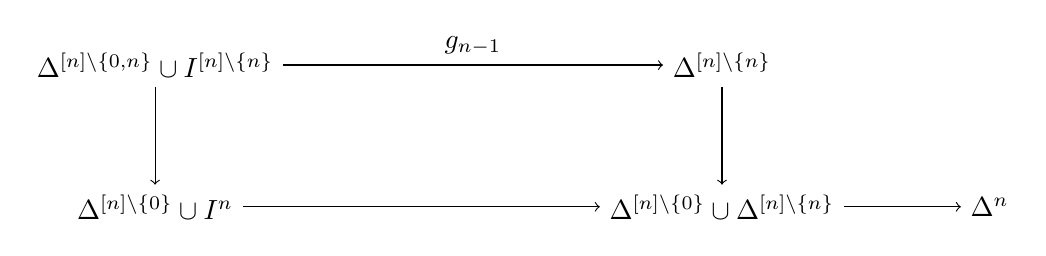
\begin{tikzpicture}
  \node (tl) at (0,0)
    {$\Delta^{[n]\setminus\{0,n\}} \cup I^{[n]\setminus\{n\}}$};
  \node (tr) at (7.2,0) {$\Delta^{[n]\setminus\{n\}}$};
  \node (bl) at (0,-1.8) {$\Delta^{[n]\setminus\{0\}} \cup I^n$};
  \node (bm) at (7.2,-1.8)
    {$\Delta^{[n]\setminus\{0\}} \cup \Delta^{[n]\setminus\{n\}}$};
  \node (br) at (10.6,-1.8) {$\Delta^n$};
  \draw[->] (tl) -- node[above] {$g_{n-1}$} (tr);
  \draw[->] (tl) -- (bl);
  \draw[->] (tr) -- (bm);
  \draw[->] (bl) -- (bm);
  \draw[->] (bm) -- (br);
\end{tikzpicture}
\end{center}
其中上面的水平映射由归纳是\trInnerAnodyne{}的。因此，左下的水平映射也是\trInnerAnodyne{}的。右下的水平
映射由 $\Lambda^n_{[n]\setminus\{0,n\}} \subseteq \Delta^n$ 给出，由%
\cref{lem:s-horn-anodyne} 第 (4) 部分，它是\trInnerAnodyne{}的，因为 $\{0, n\}$ 不是区间。
\end{proof}

\begin{corollary}\label{cor:infinity-category-composer}
每个\trInfinityCategory{}都是一个\trComposer{}。
\end{corollary}

\begin{proof}
由\cref{prop:spine-inner-anodyne} 显然。
\end{proof}

\begin{definition}\label{def:trivial-fibration}
一个\emph{\trTrivialFibration{}}（trivial fibration）是指对\trBoundaryInclusion{}%
$\partial\Delta^n \to \Delta^n$（$n \ge 0$）满足 RLP 的映射。
\end{definition}

\begin{definition}\label{def:J}
设 $J$ 是由两个\trObject{}及其间唯一的同构所构成的\trCategory{}的\trNerve{}。
\end{definition}

\begin{observation}\label{obs:J-classifier}
由两个\trObject{}及其间唯一同构构成的\trCategory{}是\trCategory{}中同构的一个\trClassifier{}%
（classifier）。换言之，由此\trCategory{}所\trCorepresented{}那个%
\trFunctor{}，就是把每个\trCategory{}映到其同构之集的那个\trFunctor{}。

给定\trInfinityCategory{} $X$ 中的一个\trMorphism{} $f$，人们于是会想知道：在
什么情形下它的分类映射 $\Delta^1 \to X$ 能扩张到 $J$ 上。容易看出，若果真如此，
则 $f$ 是一个\trEquivalence{}（见\cref{ex:extension-over-J-equivalence}）。反之亦真：这是「∞-\trGroupoid{}是%
\trKanComplex{}」这一事实的又一个应用。（注意，映射 $\Delta^1 \to J$ 是\trAnodyne{}的。）
\end{observation}

\begin{definition}\label{def:joyal-fibration}
∞-\trCategories{}之间的一个\emph{\trJoyalFibration{}}（Joyal fibration）是一个%
\trInnerFibration{}，它此外还对映射 $\Delta^0 \to J$ 满足 RLP。
\end{definition}

\begin{construction}\label{con:angle-f-i}
设 $f\colon X \to Y$ 与 $i\colon A \to B$ 是\trSimplicialSet{}之间的映射。那么存在交换图表
\begin{center}
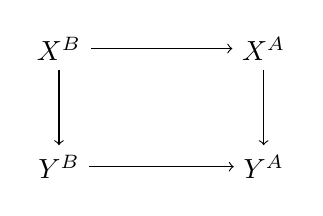
\begin{tikzpicture}
  \node (tl) at (0,0) {$X^B$};
  \node (tr) at (2.6,0) {$X^A$};
  \node (bl) at (0,-1.5) {$Y^B$};
  \node (br) at (2.6,-1.5) {$Y^A$};
  \draw[->] (tl) -- (tr);
  \draw[->] (tl) -- (bl);
  \draw[->] (tr) -- (br);
  \draw[->] (bl) -- (br);
\end{tikzpicture}
\end{center}
因此，存在诱导映射
\[
\langle f, i \rangle\colon X^B \to X^A \times_{Y^A} Y^B.
\]
\end{construction}

\begin{construction}\label{con:box-i-g}
对偶地，对\trMorphism{} $i\colon A \to B$ 与 $g\colon S \to T$，我们得到交换
图表
\begin{center}
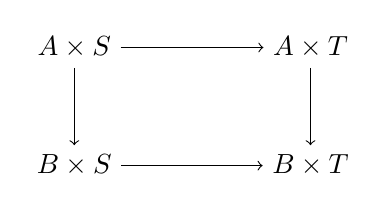
\begin{tikzpicture}
  \node (tl) at (0,0) {$A \times S$};
  \node (tr) at (3,0) {$A \times T$};
  \node (bl) at (0,-1.5) {$B \times S$};
  \node (br) at (3,-1.5) {$B \times T$};
  \draw[->] (tl) -- (tr);
  \draw[->] (tl) -- (bl);
  \draw[->] (tr) -- (br);
  \draw[->] (bl) -- (br);
\end{tikzpicture}
\end{center}
因此，存在诱导映射
\[
i \boxtimes g\colon A \times T \amalg_{A \times S} B \times S \to B \times T.
\]
\end{construction}

\begin{lemma}\label{lem:equivalent-lifting-problems}
下面两个\trLiftingProblem{}是等价的：
\begin{center}
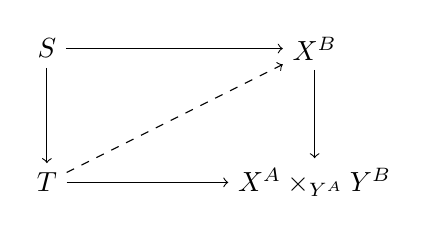
\begin{tikzpicture}
  \node (t) at (0,0) {$S$};
  \node (r) at (3.4,0) {$X^B$};
  \node (l) at (0,-1.7) {$T$};
  \node (b) at (3.4,-1.7) {$X^A \times_{Y^A} Y^B$};
  \draw[->] (t) -- (r);
  \draw[->] (t) -- (l);
  \draw[->] (l) -- (b);
  \draw[->] (r) -- (b);
  \draw[->, dashed] (l) -- (r);
\end{tikzpicture}
\hspace{3.5em}%
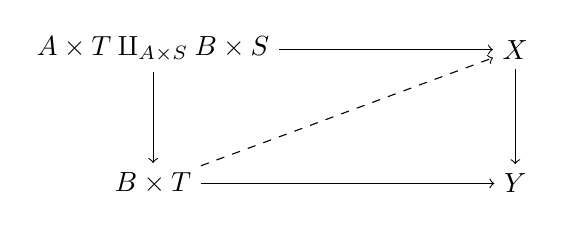
\begin{tikzpicture}
  \node (t) at (0,0) {$A \times T \amalg_{A \times S} B \times S$};
  \node (r) at (4.6,0) {$X$};
  \node (l) at (0,-1.7) {$B \times T$};
  \node (b) at (4.6,-1.7) {$Y$};
  \draw[->] (t) -- (r);
  \draw[->] (t) -- (l);
  \draw[->] (l) -- (b);
  \draw[->] (r) -- (b);
  \draw[->, dashed] (l) -- (r);
\end{tikzpicture}
\end{center}
\end{lemma}

\begin{proof}
这可以由把所有定义展开、连同\trPullback{}与\trPushout{}的泛性质、以及「\trFunctor{}%
$(-)^A$ 是\trFunctor{} $A \times -$ 的\trRightAdjoint{}」这一事实，立即得出。
\end{proof}

关于映射 $i \boxtimes g$ 的关键性技术引理如下。

\begin{lemma}\label{lem:box-anodyne}
在上述记号下，设 $i$ 与 $g$ 为\trMonomorphism{}，我们有：
\begin{enumerate}[label=(\arabic*)]
  \item $i \boxtimes g$ 是\trInnerAnodyne{}的，若 $i$ 或 $g$ 是\trInnerAnodyne{}的；
  \item $i \boxtimes g$ 是\trLeftAnodyne{}的，若 $i$ 或 $g$ 是\trLeftAnodyne{}的；
  \item $i \boxtimes g$ 是\trRightAnodyne{}的，若 $i$ 或 $g$ 是\trRightAnodyne{}的；
  \item $i \boxtimes g$ 是\trAnodyne{}的，若 $i$ 或 $g$ 是\trAnodyne{}的。
\end{enumerate}
\end{lemma}

为了证明本引理，我们需要四个以\cref{lem:box-closure} 至%
\cref{lem:left-box-generators} 为形式的预备步骤。

\begin{lemma}\label{lem:box-closure}
设 $S$ 与 $T$ 是两个由定义域皆为\trCompact{}\trMorphism{}组成的集。那么
$\overline{S} \boxtimes T \subseteq \overline{S} \boxtimes \overline{T} \subseteq \overline{S \boxtimes T}$。特别地，
\[
\overline{\overline{S} \boxtimes T} =
\overline{\overline{S} \boxtimes \overline{T}} =
\overline{S \boxtimes T}.
\]
\end{lemma}

\begin{proof}
第一个包含是显然的。为了看出第二个包含，我们令
$\mathcal{F} = \chi_R(\overline{S \boxtimes T})$。于是由%
\cref{lem:saturated-closure-equals-chi}，有
$\overline{S \boxtimes T} = \chi_L(\mathcal{F})$。现在考虑集合
$\mathcal{A} = \{\, f : f \boxtimes T \in \chi_L(\mathcal{F}) \,\}$。由%
\cref{lem:equivalent-lifting-problems}，我们有
\[
\mathcal{A} = \chi_L(\langle \mathcal{F}, T \rangle),
\]
于是由\cref{lem:chi-l-saturated} 知 $\mathcal{A}$ 是一个\trSaturatedSet{}。由于按
$\mathcal{A}$ 的定义有 $S \subseteq \mathcal{A}$，由此得出
$\overline{S} \subseteq \mathcal{A}$。这样便有
$\overline{S} \boxtimes T \subseteq \overline{S \boxtimes T}$。接下来，让我们
考虑集合 $\mathcal{B} = \{\, f : \overline{S} \boxtimes f \in \chi_L(\mathcal{F}) \,\}$。如前，我们得到
\[
\mathcal{B} = \chi_L(\langle \mathcal{F}, \overline{S} \rangle)
\]
于是 $\mathcal{B}$ 也是一个\trSaturatedSet{}。由前一步我们看到 $T \subseteq \mathcal{B}$，
因此 $\overline{T} \subseteq \mathcal{B}$ 也成立。这就证明了第一部分。对于第二
部分，我们如下论证：由于 $\overline{\overline{S} \boxtimes T}$ 是\trSaturated{}且包含
$\overline{S} \boxtimes \overline{T}$ 与 $\overline{S} \boxtimes T$，我们得到
\[
\overline{\overline{S} \boxtimes T} \subseteq
\overline{\overline{S} \boxtimes \overline{T}} \subseteq
\overline{S \boxtimes T}.
\]
另一方面，$S \boxtimes T \subseteq \overline{S} \boxtimes T \subseteq \overline{S} \boxtimes \overline{T}$，因此另一个包含也成立。
\end{proof}

\begin{lemma}\label{lem:horn-retract-box}
对 $0 < j < n$，包含 $\Lambda^n_j \to \Delta^n$ 是映射
\[
\Lambda^n_j \times \Delta^2 \amalg_{\Lambda^n_j \times \Lambda^2_1}
\Delta^n \times \Lambda^2_1 \to \Delta^n \times \Delta^2
\]
的一个收缩。
\end{lemma}

\begin{proof}
对于第一部分，考虑映射
\[
[n] \xrightarrow{\ s\ } [n] \times [2] \xrightarrow{\ r\ } [n]
\]
其中
\[
s(i) =
\begin{cases}
(i, 0) & \text{若 } i < j,\\
(i, 1) & \text{若 } i = j,\\
(i, 2) & \text{若 } i > j,
\end{cases}
\]
并且
\[
r(i, k) =
\begin{cases}
i & \text{若 } i < j \text{ 且 } k = 0,\\
i & \text{若 } i > j \text{ 且 } k = 2,\\
j & \text{其余情形。}
\end{cases}
\]
我们现在要证明：
\begin{enumerate}[label=(\arabic*)]
  \item $rs = \mathrm{id}$；
  \item $s(\Lambda^n_j) \subseteq \Lambda^n_j \times \Delta^2 \cup \Delta^n \times \Lambda^2_1$；并且
  \item $r(\Lambda^n_j \times \Delta^2 \cup \Delta^n \times \Lambda^2_1) \subseteq \Lambda^n_j$。
\end{enumerate}
（1）是一个直接的验证。为了看出（2），我们观察到事实上
$s(\Lambda^n_j) \subseteq \Lambda^n_j \times \Delta^2$：为此，只需注意到把 $s$
与投射 $[n] \times [2] \to [n]$ 复合是恒等即可。对于（3），我们需要证明两件事：
\begin{enumerate}[label=(\alph*)]
  \item $r(\Lambda^n_j \times \Delta^2) \subseteq \Lambda^n_j$，并且
  \item $r(\Delta^n \times \Lambda^2_1) \subseteq \Lambda^n_j$。
\end{enumerate}
为了证明（a），考虑 $\Lambda^n_j$ 的一个 $k$-\trSimplex{}，即 $f\colon [k] \to [n]$
使得存在 $m \in [n] \setminus \{j\}$ 不在 $f$ 的像之中，并考虑 $\Delta^2$ 的
任意一个 $k$-\trSimplex{} $\alpha\colon [k] \to [2]$。那么复合
\[
[k] \to [n] \times [2] \xrightarrow{\ r\ } [n]
\]
容易看出把 $i \in [k]$ 送到 $f(i)$ 或 $j$。于是它的像包含在 $f$ 的像与
$\{j\}$ 之并中。特别地，$m$ 不在这个复合的像中，因而它表示 $\Lambda^n_j$ 的
一个 $k$-\trSimplex{}。为了看出（b），再考虑 $\Delta^n$ 的一般 $k$-\trSimplex{}%
$\beta\colon [k] \to [n]$ 与 $\Lambda^2_1$ 的一个 $k$-\trSimplex{}%
$f\colon [k] \to [2]$，也就是说，$0$ 或 $2$ 不在 $f$ 的像中。为确定起见，设
$2$ 不在像中。（另一种情形类似。）我们发现复合
\[
[k] \xrightarrow{(\beta, f)} [n] \times [2] \xrightarrow{\ r\ } [n]
\]
把 $i \in [k]$ 送到 $\beta(i)$（若 $\beta(i) < j$）或 $j$（其余情形）。于是像
包含在 $\{0, \dotsc, j\}$ 之中。现在由于 $0 < j < n$，我们看到 $n$ 不在像中，
从而上述复合表示 $\Lambda^n_j$ 的一个 $k$-\trSimplex{}。在 $0$ 不在 $f$ 的像中的情形，
由类似的论证可知 $0$ 不在像中。这就证明了本引理。
\end{proof}

下述引理对应于 \cite[Proposition 2.3.2.1]{Lur09}。

\begin{lemma}\label{lem:inner-box-generators}
下述诸\trMorphism{}之集都生成\trInnerAnodyne{}映射之集：
\begin{enumerate}[label=(\arabic*)]
  \item 内\trHornInclusion{} $S_1 = \{\Lambda^n_j \to \Delta^n\}$（对所有
  $n \ge 2$）；
  \item 映射 $S_2 = \{(K \to L) \boxtimes (i\colon \Lambda^2_1 \to \Delta^2)\}$（对所有\trMonomorphism{} $K \to L$）；
  \item 映射 $S_3 = \{(\partial\Delta^n \to \Delta^n) \boxtimes (i\colon \Lambda^2_1 \to \Delta^2)\}$（对所有 $n \ge 0$）；
  \item 映射 $S_4 = \{(K \to L) \boxtimes (\Lambda^n_j \to \Delta^n)\}$
  （对所有\trMonomorphism{} $K \to L$ 与所有内\trHorn{}）。
\end{enumerate}
\end{lemma}

\begin{proof}
让我们先引入一些更多的记号：把\trMonomorphism{}之集记作 $T_2$，把\trBoundaryInclusion{}之集
记作 $T_3$。于是，我们有 $S_2 = T_2 \boxtimes i$、$S_3 = T_3 \boxtimes i$ 以及
$S_4 = T_2 \boxtimes S_1$。\cref{ex:chi-boundary-inclusions} 中证明了
$\overline{T_2} = \overline{T_3}$。因此，由\cref{lem:box-closure} 得出
\[
\overline{S_3} = \overline{T_3 \boxtimes i} =
\overline{\overline{T_3} \boxtimes i} =
\overline{\overline{T_2} \boxtimes i} =
\overline{T_2 \boxtimes i} = \overline{S_2}.
\]
平凡地，我们有 $\overline{S_2} \subseteq \overline{S_4}$，因为
$S_2 \subseteq S_4$。我们还发现
$\overline{S_1} \subseteq \overline{S_2} = \overline{T_2 \boxtimes i}$，因为
由\cref{lem:horn-retract-box}，任何内\trHornInclusion{}都是 $S_2$ 中某个映射的
收缩。现在注意 $T_2 \boxtimes T_2 = T_2$，于是我们额外得到
\[
\overline{S_4} = \overline{T_2 \boxtimes S_1} \subseteq
\overline{\overline{T_2} \boxtimes \overline{T_2 \boxtimes i}} =
\overline{\overline{T_2} \boxtimes \overline{T_2} \boxtimes i} =
\overline{T_2 \boxtimes i} = \overline{S_2},
\]
从而 $\overline{S_2} = \overline{S_4}$。一旦我们能证明
$\overline{S_3} \subseteq \overline{S_1}$，本引理即得证；为此，只需证明
$S_3 \subseteq \overline{S_1}$。为了这个目的，设 $m \ge 0$ 并考虑包含
\[
\Delta^m \times \Lambda^2_1 \cup \partial\Delta^m \times \Delta^2
\subseteq \Delta^m \times \Delta^2.
\]
若 $m = 0$，则该映射由 $\Lambda^2_1 \to \Delta^2$ 给出，从而是\trInnerAnodyne{}的。于是
设 $m \ge 1$。我们将如下构造 $\Delta^m \times \Delta^2$ 的一个滤过：对
$0 \le i \le j < m$，考虑 $\Delta^m \times \Delta^2$ 的那些 $(m+1)$-\trSimplex{}%
\[
\sigma_{i,j}(k) =
\begin{cases}
(k, 0) & \text{若 } 0 \le k \le i,\\
(k - 1, 1) & \text{若 } i + 1 \le k \le j + 1,\\
(k - 1, 2) & \text{若 } j + 2 \le k \le m + 1,
\end{cases}
\]
而对 $0 \le i \le j \le m$，考虑 $\Delta^m \times \Delta^2$ 的由下式给出的
$(m+2)$-\trSimplex{}%
\[
\tau_{i,j}(k) =
\begin{cases}
(k, 0) & \text{若 } 0 \le k \le i,\\
(k - 1, 1) & \text{若 } i + 1 \le k \le j + 1,\\
(k - 2, 2) & \text{若 } j + 2 \le k \le m + 2.
\end{cases}
\]
我们观察到，$\Delta^m \times \Delta^2$ 的非退化 $k$-\trSimplex{}对应于格子
$[m] \times [2]$ 中长度为 $k$、且「不在任何一点处驻足停留」的那些路径，也就是
说，它们恰好是单射映射 $[k] \to [m] \times [2]$。我们断言：
\begin{enumerate}[label=(\arabic*)]
  \item 诸\trSimplex{} $\tau_{i,j}$ 就是 $\Delta^m \times \Delta^2$ 的非退化
  $(m+2)$-\trSimplex{}：必然地，与非退化 $(m+2)$-\trSimplex{}相对应的路径必须从 $(0, 0)$ 出发
  并终止于 $(m, 2)$，只有这样才可能存在单射映射 $[m+2] \to [m] \times [2]$；
  \item 诸\trSimplex{} $\sigma_{i,j}$ 是非退化的；
  \item \trSimplex{} $\sigma_{i,j}$ 是 $\tau_{i,j}$ 与 $\tau_{i,j+1}$ 的面，但不是我们
  刚才构造的其他 $\tau$ 的面；
  \item 诸\trSimplex{} $\sigma_{i,j}$ 与 $\tau_{i,j}$ 不含于
  $\Delta^m \times \Lambda^2_1 \cup \partial\Delta^m \times \Delta^2$。
\end{enumerate}
（1）与（2）由前述观察来看是显然的。（3）由定义立即得出，（4）也是直截了当的：
投射 $[m] \times [2] \to [m]$ 把所论\trSimplex{}送到满射，因此它们不含于
$\partial\Delta^m \times \Delta^2$；同样地，投射 $[m] \times [2] \to [2]$ 也把
所论\trSimplex{}送到满射，因此它们也不含于 $\Delta^m \times \Lambda^2_1$。

现在让我们归纳地定义\trSimplicialSet{} $X(i, j)$（$0 \le i \le j < m$）如下：
\[
X(0, 0) = \Delta^m \times \Lambda^2_1 \cup \partial\Delta^m \times \Delta^2.
\]
对固定的 $j$，我们对 $i \le j < m$ 归纳地定义
\[
X(i + 1, j) = X(i, j) \cup \sigma_{i,j},
\]
并令
\[
X(0, j + 1) = X(j + 1, j).
\]
然后我们定义 $Y(0, 0) = X(0, m)$，再对 $i \le j \le m$ 归纳地定义
\[
Y(i + 1, j) = Y(i, j) \cup \tau_{i,j},
\]
并令
\[
Y(0, j + 1) = Y(j + 1, j).
\]
由于诸 $\tau_{i,j}$ 就是 $\Delta^m \times \Delta^2$ 的非退化 $(m+2)$-\trSimplex{}，我们
发现 $Y(0, m + 1) = \Delta^m \times \Delta^2$。为了完成本引理的证明，我们必须
证明下述陈述：
\begin{enumerate}[label=(\Alph*)]
  \item \trSimplicialSet{} $X(i, j) \cap \sigma_{i,j}$ 是一个内\trHorn{}。
  \item \trSimplicialSet{} $Y(i, j) \cap \tau_{i,j}$ 是一个内\trHorn{}。
\end{enumerate}
由此得出，所有映射 $X(i, j) \to X(i + 1, j)$ 与所有映射
$Y(i, j) \to Y(i + 1, j)$ 都是\trInnerAnodyne{}的：在两种情形下，它们都是内\trHornInclusion{}的%
\trPushout{}，这正是它们的复合 $X(0, 0) \to Y(0, m+1)$ 也是\trInnerAnodyne{}的原因，引理
随之得证。

\begin{itemize}
\item (A) 的证明：我们必须证明，对所有 $0 \le i \le j < m$，映射
\[
[m + 1] \xrightarrow{\ \sigma_{i,j}\ } [m] \times [2]
\]
把所有 $m$ 维面都送到 $X(i, j)$ 中，唯独一个内 $m$ 维面除外。我们断言，
$\sigma_{i,j}$ 的 $(i+1)$-面就是那个不含于 $X(i, j)$ 的面。注意
$0 < i + 1 < m + 1$，于是 $\sigma_{i,j} \cap X(i, j)$ 是一个内\trHorn{}。
$\sigma_{i,j}$ 只有两个面不含于 $\partial\Delta^m \times \Delta^2 \subseteq X(0, 0)$，即与那条唯一的竖直边相毗邻、组成水平边的那些面。它们是
$d_i\sigma_{i,j}$ 与 $d_{i+1}\sigma_{i,j}$，因此只需验证 $d_i\sigma_{i,j}$ 含于
$X(i, j)$，而 $d_{i+1}\sigma_{i,j}$ 不含于 $X(i, j)$。前一个陈述很容易看出：
只要 $i > 0$，就有 $d_i\sigma_{i-1,j} = d_i\sigma_{i,j}$，而 $d_0\sigma_{0,j}$
含于 $\Delta^m \times \Lambda^2_1$，因为投影到 $[2]$ 之后 $0$ 不在像中。剩下要
证明后一个陈述，即 $d_{i+1}\sigma_{i,j}$ 不含于 $X(i, j)$。我们已经看到
$d_{i+1}\sigma_{i,j}$ 不含于 $\partial\Delta^m \times \Delta^2$。因此，我们
需要证明：
\begin{enumerate}[label=(\arabic*)]
  \item $d_{i+1}\sigma_{i,j}$ 不含于 $\Delta^m \times \Lambda^2_1$；
  \item $d_{i+1}\sigma_{i,j}$ 不含于 $\sigma_{k,j}$（$k < i$）；并且
  \item $d_{i+1}\sigma_{i,j}$ 不含于 $\sigma_{k,l}$（$k \le l < j$）。
\end{enumerate}
（1）由 $0 < i + 1 < m + 1$ 这一事实得出，也就是说，在投影
$[m] \times [2] \to [2]$ 之后，$0$ 与 $2$ 都在 $d_{i+1}\sigma_{i,j}$ 的像中。
对于（2），我们观察到与 $d_{i+1}\sigma_{i,j}$ 相对应的路径经过点 $(i, 0)$，而
对 $\sigma_{k,j}$（$k < i$）情形并非如此，从而对其任何面也非如此。同样地，若
$i < j$，则 $d_{i+1}\sigma_{i,j}$ 经过点 $(j, 1)$，而对任何 $\sigma_{k,l}$
（$l < j$）情形并非如此。若 $i = j$，则 $d_{i+1}\sigma_{i,j}$ 再次经过
$(i, 0)$，而对 $\sigma_{k,l}$（$k \le l < j = i$）情形并非如此，于是像第一种
情形那样有 $k < i$。

\item (B) 的证明：同样，我们断言 $d_{i+1}\tau_{i,j}$ 是唯一不含于 $Y(i, j)$
的面。

（a）我们先考虑 $i < j$ 的情形。再次观察可知，$d_\ell\tau_{i,j}$ 含于
$\partial\Delta^m \times \Delta^2$，除非 $\ell \in \{i, i + 1, j + 1, j + 2\}$；
并且 $d_{j+1}\tau_{i,j} = \sigma_{i,j-1}$、$d_{j+2}\tau_{i,j} = \sigma_{i,j}$，
因此这二者都含于 $Y(i, j)$。同样地，若 $i > 0$，则
$d_i\tau_{i,j} = d_i\tau_{i-1,j}$，因此这个面也含于 $Y(i, j)$。若 $i = 0$，则
$d_i\tau_{i,j}$ 含于 $\Delta^m \times \Lambda^2_1$，\footnote{译注：原书此处
印作「$\Delta^m \cup \Lambda^2_1$」，按上下文应为
$\Delta^m \times \Lambda^2_1$。}因为其到 $[2]$ 的投影的像中不含 $0$。现在我们
证明 $d_{i+1}\tau_{i,j}$ 不含于 $Y(i, j)$，这意味着
$Y(i, j) \cap \tau_{i,j}$ 又是一个内\trHorn{}（因为 $0 < i + 1 < m + 2$）。与
情形 (A) 中一样，我们需要看出：
\begin{enumerate}[label=(\arabic*)]
  \item $d_{i+1}\tau_{i,j}$ 不含于 $\tau_{k,j}$（$k < i$）；并且
  \item $d_{i+1}\tau_{i,j}$ 不含于 $\tau_{k,l}$（$k \le l < j$）。
\end{enumerate}
如前，$d_{i+1}\tau_{i,j}$ 经过点 $(i, 0)$，而对 $\tau_{k,j}$（$k < i$）情形并非
如此。同样地，$d_{i+1}\tau_{i,j}$ 经过点 $(j, 1)$，而对 $\tau_{k,l}$
（$l < j$）情形并非如此。

（b）最后，我们考虑 $i = j$ 的情形。我们断言，$d_{i+1}\tau_{i,i}$ 仍是唯一不含
于 $Y(i, i)$ 的面。若 $i = j = 0$，则 $d_0\tau_{0,0}$ 含于
$\Delta^m \times \Lambda^2_1$，因为其到 $[2]$ 的投影错过了 $0$。若 $i > 0$，
则我们有 $d_i\tau_{i,i} = d_i\tau_{i-1,i}$，因此 $d_i\tau_{i,i}$ 在各种情形下
都含于 $Y(i, i)$。同样地，我们有 $d_{i+2}\tau_{i,i} = \sigma_{i,i}$。若
$l < i$ 或 $l > i + 2$，则 $d_l\tau_{i,i}$ 到 $[m]$ 的投影不是满射，从而
$d_l\tau_{i,i}$ 含于 $\partial\Delta^m \times \Delta^2$。剩下要证明：
\begin{enumerate}[label=(\arabic*)]
  \item $d_{i+1}\tau_{i,i}$ 不含于 $\tau_{k,j}$（$k < i$）；并且
  \item $d_{i+1}\tau_{i,i}$ 不含于 $\tau_{k,l}$（$k \le l < j$）。
\end{enumerate}
注意，在这两种情形都有 $k < i$，而且 $d_{i+1}\tau_{i,i}$ 经过点 $(i, 0)$。但是，
无论 $l$ 是什么，$\tau_{k,l}$ 都不经过 $(i, 0)$。
\end{itemize}
\end{proof}

\begin{lemma}\label{lem:left-box-generators}
下述诸\trMorphism{}之集都生成左\trAnodyne{}映射之集：
\begin{enumerate}[label=(\arabic*)]
  \item 左\trHornInclusion{} $S_1 = \{\Lambda^n_j \to \Delta^n\}$（对所有
  $n \ge 1$ 与 $0 \le j < n$）；
  \item 映射 $S_2 = \{(K \to L) \boxtimes (i\colon \{0\} \to \Delta^1)\}$
  （对所有\trMonomorphism{} $K \to L$）；
  \item 映射 $S_3 = \{(\partial\Delta^n \to \Delta^n) \boxtimes (i\colon \{0\} \to \Delta^1)\}$（对所有 $n \ge 0$）；
  \item 映射 $S_4 = \{(K \to L) \boxtimes (\Lambda^n_j \to \Delta^n)\}$
  （对所有\trMonomorphism{} $K \to L$、所有 $n \ge 1$ 与 $0 \le j < n$）。
\end{enumerate}
\end{lemma}

\begin{proof}
与\cref{lem:inner-box-generators} 的证明一样，只有下述两个陈述不能由先前的考虑
得出：
\begin{enumerate}[label=(\arabic*)]
  \item $S_3$ 中的映射是\trLeftAnodyne{}的。
  \item 映射 $\Lambda^n_j \to \Delta^n$ 是\trPushoutProduct{}（pushout product）映射
  \[
  \Delta^n \times \{0\} \amalg_{\Lambda^n_j \times \{0\}}
  \Lambda^n_j \times \Delta^1 \to \Delta^n \times \Delta^1
  \]
  的一个收缩。
\end{enumerate}
这两个陈述都包含在\cref{ex:horn-retract-pushout-product} 中。这里，我们给出如下提示：对于（1），考虑
$\Delta^n \times \Delta^1$ 的一个类似的滤过——从该\trPushoutProduct{}的定义域出发，逐步
添加 $\Delta^n \times \Delta^1$ 中缺失的非退化 $(n + 1)$-\trSimplex{}——然后照搬
\cref{lem:inner-box-generators} 中相同的论证。对于（2），考虑映射
\[
[n] \xrightarrow{\ s\ } [n] \times [1] \xrightarrow{\ r\ } [n],
\]
其中 $s$ 是包含 $k \mapsto (k, 1)$，而
\[
r(k, i) =
\begin{cases}
k & \text{若 } k \ne j + 1 \text{ 且 } i = 0,\\
j & \text{若 } (k, i) = (j + 1, 0),\\
k & \text{若 } i = 1.
\end{cases}
\]
\end{proof}

\begin{corollary}\label{cor:right-box-generators}
下述诸\trMorphism{}之集都生成右\trAnodyne{}映射之集：
\begin{enumerate}[label=(\arabic*)]
  \item 右\trHornInclusion{} $S_1 = \{\Lambda^n_j \to \Delta^n\}$（对所有
  $n \ge 1$ 与 $0 < j \le n$）；
  \item 映射 $S_2 = \{(K \to L) \boxtimes (i\colon \{1\} \to \Delta^1)\}$
  （对所有\trMonomorphism{} $K \to L$）；
  \item 映射 $S_3 = \{(\partial\Delta^n \to \Delta^n) \boxtimes (i\colon \{1\} \to \Delta^1)\}$（对所有 $n \ge 0$）；
  \item 映射 $S_4 = \{(K \to L) \boxtimes (\Lambda^n_j \to \Delta^n)\}$
  （对所有\trMonomorphism{} $K \to L$、所有 $n \ge 1$ 与 $0 < j \le n$）。
\end{enumerate}
\end{corollary}

\begin{proof}
我们观察到，一个映射是\trRightAnodyne{}的当且仅当它的相反映射（opposite）是\trLeftAnodyne{}的，
这是因为根据\cref{ex:inner-fibration-op}，一个映射是左纤维化当且仅当其相反映射是右纤维化。于是，
第一部分由 $(\Lambda^n_j)^{\mathrm{op}} \cong \Lambda^n_{n-j}$ 这一事实、以及
「所涉及的诸\trSimplicialSet{}的所有其他\trMorphism{}都是『自相反的』（self-opposite）」
这一事实得出。
\end{proof}

\begin{proof}[\cref{lem:box-anodyne} 的证明]
第 (1) 部分由\cref{lem:inner-box-generators} 中的等式
$\overline{S_4} = \overline{S_1}$ 得出，第 (2) 部分由%
\cref{lem:left-box-generators} 中的等式 $\overline{S_4} = \overline{S_1}$
得出，而第 (3) 部分由\cref{cor:right-box-generators} 中的等式
$\overline{S_4} = \overline{S_1}$ 得出。为了看出第 (4) 部分，我们简单地观察
到：\trAnodyneMap{}由左\trAnodyne{}映射与右\trAnodyne{}映射生成（作为一个\trSaturatedSet{}）。因此，只需证明：
当 $i$ 是\trLeftAnodyne{}（相应地，\trRightAnodyne{}）映射而 $g$ 是\trMonomorphism{}时，
$i \boxtimes g$ 是\trAnodyne{}的。由于\trLeftAnodyne{}（相应地，\trRightAnodyne{}）映射是\trAnodyne{}的，这一点
分别由陈述 (2) 与 (3) 得出。
\end{proof}

\begin{theorem}\label{thm:angle-fi-fibration}
设 $f\colon X \to Y$ 是一个（内、左、右）纤维化，并设 $i\colon A \to B$ 是一个%
\trMonomorphism{}。那么：
\begin{enumerate}[label=(\arabic*)]
  \item 映射 $\langle f, i \rangle$ 是一个（内、左、右）纤维化。
  \item 若此外 $i$ 还是（内、左、右）\trAnodyne{}的，则映射
  $\langle f, i \rangle$ 是一个\trTrivialFibration{}。
\end{enumerate}
\end{theorem}

\begin{proof}
我们先证 (1)。为此，考虑\trLiftingProblem{}%
\begin{center}
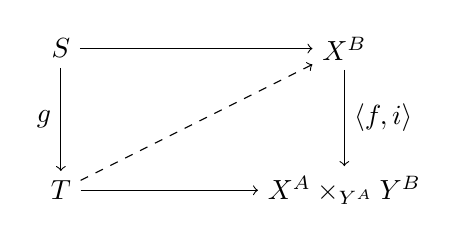
\begin{tikzpicture}
  \node (t) at (0,0) {$S$};
  \node (r) at (3.6,0) {$X^B$};
  \node (l) at (0,-1.8) {$T$};
  \node (b) at (3.6,-1.8) {$X^A \times_{Y^A} Y^B$};
  \draw[->] (t) -- (r);
  \draw[->] (t) -- node[left] {$g$} (l);
  \draw[->] (l) -- (b);
  \draw[->] (r) -- node[right] {$\langle f, i \rangle$} (b);
  \draw[->, dashed] (l) -- (r);
\end{tikzpicture}
\end{center}
其中映射 $g\colon S \to T$ 是（内、左、右）\trAnodyne{}的。由%
\cref{lem:equivalent-lifting-problems}，求解这个问题等价于求解\trLiftingProblem{}%
\begin{center}
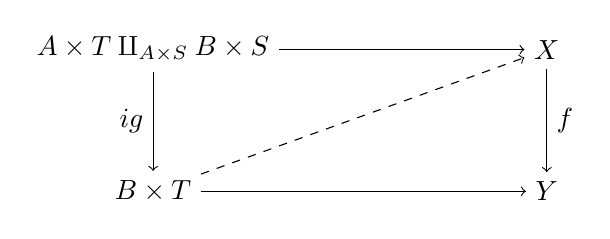
\begin{tikzpicture}
  \node (t) at (0,0) {$A \times T \amalg_{A \times S} B \times S$};
  \node (r) at (5,0) {$X$};
  \node (l) at (0,-1.8) {$B \times T$};
  \node (b) at (5,-1.8) {$Y$};
  \draw[->] (t) -- (r);
  \draw[->] (t) -- node[left] {$i \boxtimes g$} (l);
  \draw[->] (l) -- (b);
  \draw[->] (r) -- node[right] {$f$} (b);
  \draw[->, dashed] (l) -- (r);
\end{tikzpicture}
\end{center}
由\cref{lem:box-anodyne}，我们知道 $i \boxtimes g$ 是（内、左、右）\trAnodyne{}的，而由
假设，$f$ 是一个（内、左、右）纤维化。

为了证明 (2)，我们需要像上面那样再考虑一个\trLiftingProblem{}，不过此时 $g$ 是一个%
\trMonomorphism{}。由于 $i$ 是（内、左、右）\trAnodyne{}的，我们同样看到，由%
\cref{lem:box-anodyne} 可以求解这个\trLiftingProblem{}。
\end{proof}

\begin{corollary}\label{cor:functor-kan}
设 $K$ 与 $X$ 是\trSimplicialSet{}。若 $X$ 是一个\trInfinityCategory{}，那么 $X^K$ 也是。若
$X$ 是一个\trKanComplex{}，那么 $X^K$ 也是。
\end{corollary}

\begin{proof}
这是\cref{thm:angle-fi-fibration} 第 (1) 部分的一个特例，其中 $A$ 为空、$B = K$
且 $Y = \Delta^0$。
\end{proof}

\begin{definition}\label{def:functor-infinity-category}
设 $\C$ 与 $\D$ 是\trInfinityCategories{}。我们把从 $\C$ 到
$\D$ 的\trFunctor{}∞-范畴定义为
$\mathrm{Fun}(\C, \D) = \underline{\mathrm{Hom}}(\C, \D)$。
由\cref{cor:functor-kan}，它是一个\trInfinityCategory{}。
\end{definition}

\begin{observation}\label{obs:fun-simplices}
再次注意，$\mathrm{Fun}(\C, \D)$ 的 $0$-\trSimplex{}与 $1$-\trSimplex{}正是%
\cref{def:functor-infinity-categories} 与定义 1.2.79 中所定义的\trFunctor{}与%
\trNaturalTransformation{}。

此外，若 $\D$ 是一个\trKanComplex{}，则
$\mathrm{Fun}(\C, \D)$ 本身是一个\trKanComplex{}，从而特别地是一个
∞-\trGroupoid{}。这一点与「∞-\trGroupoid{}是\trKanComplex{}」这一（有待证明）
的事实一道，暗示在\trFunctor{}范畴中，逐点为\trEquivalence{}的\trMorphism{}事实
上是一个\trEquivalence{}。这将被证明是对的，但
证明起来会更加复杂，其难度超过证明「\trKanComplex{}恰好就是∞-\trGroupoid{}」，
见定理 2.2.1。
\end{observation}

我们现在已有条件给出空间∞-范畴的一个新定义，它是纯单纯的。

\begin{definition}\label{def:spc-hat}
我们考虑\trSimplicialCategory{} $\mathrm{Kan}$，其\trObject{}由诸\trKanComplex{} $X$ 给出，
而从 $X$ 到 $Y$ 的 hom-\trSimplicialSet{}由内 hom-\trSimplicialSet{}%
$\underline{\mathrm{Hom}}(X, Y)$ 给出。我们令
$\widehat{\mathrm{Spc}} = \mathrm{N}(\mathrm{Kan})$ 为其\trCoherentNerve{}。
\end{definition}

\begin{observation}\label{obs:canonical-spc-hat}
存在一个典范\trFunctor{} $\mathrm{Spc} \to \widehat{\mathrm{Spc}}$。为了构造
这个单纯\trFunctor{}，回忆 $\mathrm{Spc}$ 是 CW 复形的\trSimplicialCategory{}的%
\trCoherentNerve{}，如\cref{def:infinity-category-spaces} 中那样。我们断言：
把 CW 复形 $X$ 送到它的奇异复形 $\mathcal{S}(X)$ 就诱导出所需的单纯%
\trFunctor{}。为此，我们需要证明存在\trSimplicialSet{}的一个典范映射
\[
\mathcal{S}(\mathrm{map}(X, Y)) \to
\underline{\mathrm{Hom}}(\mathcal{S}(X), \mathcal{S}(Y))
\]
它与复合相容。这个映射构造如下：由\trAdjunction{}性，只需构造一个映射
\[
\mathcal{S}(\mathrm{map}(X, Y)) \times \mathcal{S}(X) \to \mathcal{S}(Y).
\]
利用「$\mathcal{S}$（作为一个\trRightAdjoint{}）与积交换」，这等价地由一个
典范映射
\[
\mathcal{S}(\mathrm{map}(X, Y) \times X) \to \mathcal{S}(Y)
\]
提供。现在我们使用连续的求值映射
$\mathrm{map}(X, Y) \times X \to Y$，并把\trFunctor{} $\mathcal{S}$ 应用到其
上。不难看出，如此得到的映射与复合相容，因而如所断言，确定了一个\trFunctor{}%
$\mathrm{Spc} \to \widehat{\mathrm{Spc}}$。
\end{observation}

\begin{observation}\label{obs:spc-hat-weak-equivalence}
此外，我们断言映射
\[
\mathcal{S}(\mathrm{map}(X, Y)) \to
\underline{\mathrm{Hom}}(\mathcal{S}(X), \mathcal{S}(Y))
\]
是一个\trWeakEquivalence{}，因此从 CW 复形到\trKanComplex{}的单纯\trFunctor{}%
在\cref{def:weak-equivalence-simplicial} 的意义下是一个\trWeakEquivalence{}。
在本书稍后的阶段，我们将证明：Kan 充实的\trSimplicialCategory{}之间的\trWeakEquivalence{}在
施加\trCoherentNerve{}之后诱导∞-\trCategories{}之间的\trEquivalence{}，从而，
我们所定义的两个空间∞-范畴事实上是等价的。
\end{observation}

\begin{corollary}\label{cor:trivial-fibration-characterization}
\trSimplicialSet{} $\C$ 是一个\trInfinityCategory{}，当且仅当典范映射
$\C^{\Delta^2} \to \C^{\Lambda^2_1}$ 是一个\trTrivialFibration{}。特别地，对一个%
\trInfinityCategory{} $\C$，在固定图表 $\Lambda^2_1 \to \C$ 之上的纤维是一个
可缩的\trKanComplex{}。
\end{corollary}

\begin{proof}
「仅当」部分由「$\Lambda^2_1 \to \Delta^2$ 是\trInnerAnodyne{}的」、「$\C \to \ast$ 是一个%
\trInnerFibration{}」以及\cref{thm:angle-fi-fibration} 得出。为了看出反之亦然，
我们希望证明：若 $\C^{\Delta^2} \to \C^{\Lambda^2_1}$ 是一个\trTrivialFibration{}，则
$\C \to \ast$ 是一个\trInnerFibration{}。

为了证明 $\C \to \ast$ 是一个\trInnerFibration{}，由%
\cref{lem:inner-box-generators}，只需证明它对 $S_2$ 中的映射容许扩张性质。由%
\trAdjunction{}性，这成立当且仅当 $\C^{\Delta^2} \to \C^{\Lambda^2_1}$ 对所有%
\trMonomorphism{}满足扩张性质，而这成立当且仅当它是一个\trTrivialFibration{}。

对于「特别地」部分，考虑 $\C$ 中两个可合成的\trMorphism{} $f$ 与 $g$，并把它
们视为一个映射 $\Lambda^2_1 \to \C$。那么在\trPullback{}图表
\begin{center}
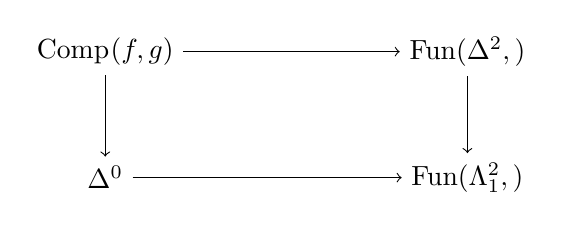
\begin{tikzpicture}
  \node (tl) at (0,0) {$\mathrm{Comp}_{\C}(f, g)$};
  \node (tr) at (4.6,0) {$\mathrm{Fun}(\Delta^2, \C)$};
  \node (bl) at (0,-1.6) {$\Delta^0$};
  \node (br) at (4.6,-1.6) {$\mathrm{Fun}(\Lambda^2_1, \C)$};
  \draw[->] (tl) -- (tr);
  \draw[->] (tl) -- (bl);
  \draw[->] (tr) -- (br);
  \draw[->] (bl) -- (br);
\end{tikzpicture}
\end{center}
中，右边的竖直映射是一个\trTrivialFibration{}，因此左边的竖直映射也是\trTrivialFibration{}。特别地，
对任意两个可合成的\trMorphism{}，由诸合成构成的\trSimplicialSet{}%
$\mathrm{Comp}_{\C}(f, g)$ 是一个可缩的\trKanComplex{}。
\end{proof}

\begin{remark}\label{rem:spine-trivial-fibration}
同一套论证表明：对一个\trInfinityCategory{} $\C$，映射
$\C^{\Delta^n} \to \C^{I^n}$ 对所有 $n \ge 2$ 都是\trTrivialFibration{}，因为映射
$I^n \to \Delta^n$ 是\trInnerAnodyne{}的。
\end{remark}

\begin{lemma}\label{lem:trivial-fibration-section}
任何\trTrivialFibration{} $X \to Y$ 都容许一个\trSectionMap{}，而且这些\trSectionMap{}汇集起来构成一个可缩的%
\trKanComplex{}。
\end{lemma}

\begin{proof}
对任意\trSimplicialSet{} $A$，映射
$\underline{\mathrm{Hom}}(A, X) \to \underline{\mathrm{Hom}}(A, Y)$\footnote{译注：原书印作
$\mathrm{Hom}(A, X)$（无下划线），按义应为内 hom，此处径改。}仍是一个%
\trTrivialFibration{}。特别地，取 $A = Y$ 时正是如此。那么在 $\mathrm{id}_Y$ 之上的纤维
是一个可缩的\trKanComplex{}，其零\trSimplex{}恰是 $p$ 的\trSectionMap{}。
\end{proof}

由于前一个引理，我们可以选取上述\trTrivialFibration{}的一个\trSectionMap{}，并得到复合
\[
\C^{\Lambda^2_1} \to \C^{\Delta^2} \to \C^{\Delta^{\{0,2\}}}
\]
把它当作∞-\trCategories{}的\trFunctor{}（即\trSimplicialSet{}之间的映射）。由于第一个\trCategory{}%
等价于 $\C^{\Delta^1} \times_{\C} \C^{\Delta^1}$（其中两个映射分别为目标与
源），我们便得到一个在∞-\trCategory{} $\C$ 中编码合成的\trFunctor{}：
\[
\C^{\Delta^1} \times_{\C} \C^{\Delta^1} \to \C^{\Delta^1}
\]

\begin{definition}\label{def:mapping-infinity-category}
设 $\C$ 是一个\trInfinityCategory{}，并设 $x, y \in \C$ 是\trObject{}。那么，
我们把 $x$ 与 $y$ 之间的映射∞-范畴定义为如下\trPullback{}%
\begin{center}
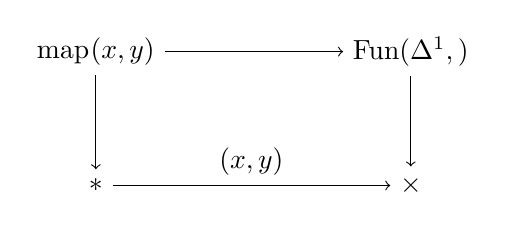
\begin{tikzpicture}
  \node (tl) at (0,0) {$\mathrm{map}_{\C}(x, y)$};
  \node (tr) at (4,0) {$\mathrm{Fun}(\Delta^1, \C)$};
  \node (bl) at (0,-1.7) {$\ast$};
  \node (br) at (4,-1.7) {$\C \times \C$};
  \draw[->] (tl) -- (tr);
  \draw[->] (tl) -- (bl);
  \draw[->] (tr) -- (br);
  \draw[->] (bl) -- node[above] {$(x, y)$} (br);
\end{tikzpicture}
\end{center}
其中右边的竖直映射是源与目标（即在 $0$ 与 $1$ 处求值）。
\end{definition}

注意，我们容易看出 $\mathrm{map}_{\C}(x, y)$ 是一个\trInfinityCategory{}，因为由
\cref{thm:angle-fi-fibration}，映射
$\mathrm{Fun}(\Delta^1, \C) \to \C \times \C$ 是一个\trInnerFibration{}。事实
上，更多的结论成立，但我们必须把下述命题的证明推迟到本书稍后的阶段，见推论
2.2.4。

\begin{proposition}\label{prop:mapping-infinity-groupoid}
若 $\C$ 是一个\trInfinityCategory{}，则对所有\trObject{} $x, y \in \C$，
$\mathrm{map}_{\C}(x, y)$ 是一个∞-\trGroupoid{}。
\end{proposition}

因此，我们得到一个\trFunctor{}%
\[
\begin{aligned}
\mathrm{map}_{\C}(x, y) \times \mathrm{map}_{\C}(y, z) &\to
\mathrm{Fun}(\Delta^1, \C) \times_{\C} \mathrm{Fun}(\Delta^1, \C) \\
&\to \mathrm{Fun}(\Delta^1, \C)
\end{aligned}
\]
它使图表
\begin{center}
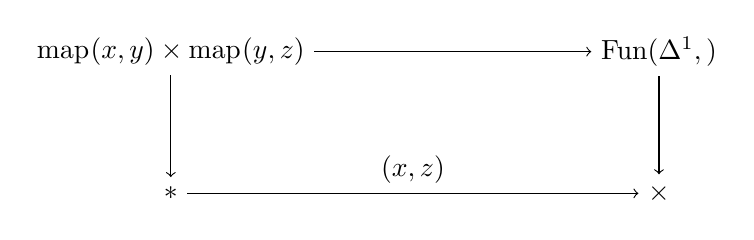
\begin{tikzpicture}
  \node (tl) at (0,0) {$\mathrm{map}_{\C}(x, y) \times \mathrm{map}_{\C}(y, z)$};
  \node (tr) at (6.2,0) {$\mathrm{Fun}(\Delta^1, \C)$};
  \node (bl) at (0,-1.8) {$\ast$};
  \node (br) at (6.2,-1.8) {$\C \times \C$};
  \draw[->] (tl) -- (tr);
  \draw[->] (tl) -- (bl);
  \draw[->] (tr) -- (br);
  \draw[->] (bl) -- node[above] {$(x, z)$} (br);
\end{tikzpicture}
\end{center}
交换。于是我们得到一个\trFunctor{}%
\[
\mathrm{map}_{\C}(x, y) \times \mathrm{map}_{\C}(y, z) \to
\mathrm{map}_{\C}(x, z)
\]
我们把它称作∞-\trCategory{} $\C$ 中的合成。
